% ==============================================================================
\chapter{CLIC: the Compact LInear Collider}
\label{ch:CLIC}
% ============================================================================== 

The energy loss due to the synchrotron radiation in a circular
accelerator limits the center-of-mass energy $\sqrt{s}$ reached by
electron beams. The energy loss is inversely proportional to the
bending radius of the accelerator and the particle mass. 

The proposed Compact Linear Collider
(CLIC)~\cite{Aicheler:1500095,Linssen:1425915}, as a future linear
particle collider for electrons (e$^-$) and positrons (e$^+$), can
avoid synchrotron radiation losses and attain higher center-of-mass
energies than the Large Electron-Positron Collider (LEP).

Today, the Large Hadron Collider (LHC) is the largest particle
accelerator being able to collide two opposing particle beams of
protons with a center-of-mass energy up to $13\,\tev$. So far, the
main result of the LHC is the observation of the Higgs boson and the
determination of its mass in 2012. However, the experiments at the LHC
can not fully answer the questions on the nature of this particle. In
the post-LHC era, CLIC will allow to determine the properties of the
Higgs boson with a very high precision. CLIC can measure collisions
with center-of-mass energies from $380\,\gev$ up to $3\,\tev$.

In this chapter, we will briefly discuss the standard model of
particle physics and attempt to understand how CLIC can determine more
precisely the properties of the Higgs boson. Then the CLIC detector
and its components are described. The focus is put on the vertex
detector, its requirements and its flavour-tagging performance.

\section{The Standard Model} 

In particle physics, the Standard Model (SM) is a theoretical
framework that describes how the interaction between elementary
particles is governed by four fundamental forces. This theory,
developed in the early 1970s, explains most of the experimental
results.

According to the Standard Model, matter is made of elementary
particles. They can be regrouped into three basic kinds: quarks,
leptons and gauge bosons as shown in~\cref{fig:standardmodel}.

\begin{figure}[htbp]
  \centering
  \includegraphics[width=0.7\textwidth]{figures/CLIC/StandardModel.png}
  \caption{The building blocks of matter according to the Standard
    Model~\cite{wikipediaParticles}.}
  \label{fig:standardmodel}
\end{figure}

Today, the Standard Model is the best theory describing the subatomic
world. However, it does not answer questions like the nature of dark
matter. This theory also predicts the existence of the Higgs boson
which gives the mass to all particles. It was experimentally observed
in 2012 by the LHC experiments.

The weak and the electromagnetic forces are closely related to each
other and can be unified as the \begin{it}electroweak\end{it} force
and the equations describing the unification predict the
force-carrying particles (the photon, the W and Z bosons). The only
problem is that all the force-carrying particles are described as
being massless which is true for the photon, but the W and Z bosons
have a mass about 100 times larger than that of the proton. To solve
this problem, the Brout-Englert-Higgs mechanism was introduced which
suggests that the Higgs boson gives the mass to the W and Z boson by
interaction with a Higgs field.

The Higgs particle can be produced in a particle collider by
accelerating particles to high energies and speed (close to the speed
of light) and colliding them together. Heavy particles, like the Higgs
boson, are occasionally produced and then detected by a particle
detector. The Standard Model predicts different mechanisms to produce
the Higgs boson and the probability to produce it is very small. For
example, in LHC only 1 Higgs boson is produced per 10 billion
collisions.

CLIC studies different mechanisms to produce the Higgs boson as shown
in \cref{fig:HiggsProductionMechanisms}.

\begin{figure}[htbp]
  \centering
  \includegraphics[page=43, trim=30mm 235mm 10mm 30mm, clip, width=0.7\textwidth]{figures/CLIC/clicCDR.pdf}
  \caption{Standard Model Higgs boson production mechanisms at
    CLIC~\cite{Linssen:1425915}.}
  \label{fig:HiggsProductionMechanisms}
\end{figure}

% The cross sections (the probability for a specific process to occur in a given interaction) to produce a Higgs with a mass of $M_H = 125$~GeV as a function of the center-of-mass energy\footnote{The center-of-mass energy is given by $\sqrt{s} = \sqrt{\left( \sum_{i}{E_i}^2 - \sum_{i}{p_i}^2 \right)}$.} $\sqrt{s}$ is given in Figure \ref{fig:corssSectionH125}. For lower $\sqrt{s}$, the HZ mechanism is dominant. For higher energies, the H$\nu_{e}\bar{\nu_{e}}$ mechanism gets dominant. 

% \begin{figure}[H]
%   \centering
%   %\hspace{2cm}
%   %% \includegraphics[page=43, trim=50mm 125mm 20mm 120mm, clip, width=0.8\textheight]{Chapters/Figures/CLIC/clicCDR.pdf}
%   %%\includegraphics[page=12, trim=50mm 190mm 20mm 30mm, clip, width=0.5\textheight]{Chapters/Figures/CLIC/clicCDR_vol3.pdf}
%   \includegraphics[width=0.3\textheight]{Chapters/Figures/CLIC/Higgs125.pdf}
%   \caption{Cross sections for different production mechanisms for a $M_H~=~125$~GeV Higgs boson as a function of the e$^+$e$^-$ center-of-mass energy. From \cite{CLICCDRvol3}.}
%   \label{fig:corssSectionH125}
% \end{figure}

Like many other particle, the Higgs boson decays quickly into a set of
lighter particles. It can decay through many different processes and
each has its own probability. As its lifetime is very small, it can
not be detected directly by the detectors. It can be recognized by the
reconstruction of its decay products in the detector. Each part of a
particle detector is optimized for detecting specific particle
properties.

An electron-positron collider allows to perform precision measurements
because the colliding beams are made of elementary particles. In fact,
with elementary particles, the center-of-mass energy and the
polarization of the colliding particles can be selected precisely. And
unlike proton-proton collisions (used in the LHC experiments), there
is no underlying event from proton remnants as shown in
\cref{fig:CLICvsLHC}. This is the reason why CLIC can do more precise
measurements on the Higgs bosons and provide complementary information
on the LHC results.

\begin{figure}[htbp]
  \centering
  \includegraphics[page=5, trim=10mm 10mm 10mm 45mm, clip, width=0.7\textwidth]{figures/CLIC/andrePresentation.pdf}
  \caption{Schematic view of electron-positron collisions at CLIC
    (left) and proton collisions at the LHC
    (right)~\cite{website:Sailer}.}
  \label{fig:CLICvsLHC}
\end{figure}

\section{The CLIC accelerator}
\label{sec:CLICaccelerator}

The CLIC accelerator is planned to be built in three various stages
with center-of-mass energies of $380\,\gev$, $1.5\,\tev$ and $3\,\tev$
as shown in \cref{fig:CLICstaging}. The site studies have shown that
CLIC could be placed near CERN underground. For each stage, to
increase the center-of-mass energy, more accelerating modules will be
needed, making the accelerator longer. The site length for
$3\,\tev$ will be 48~km.

\begin{figure}[htbp]
  \centering
  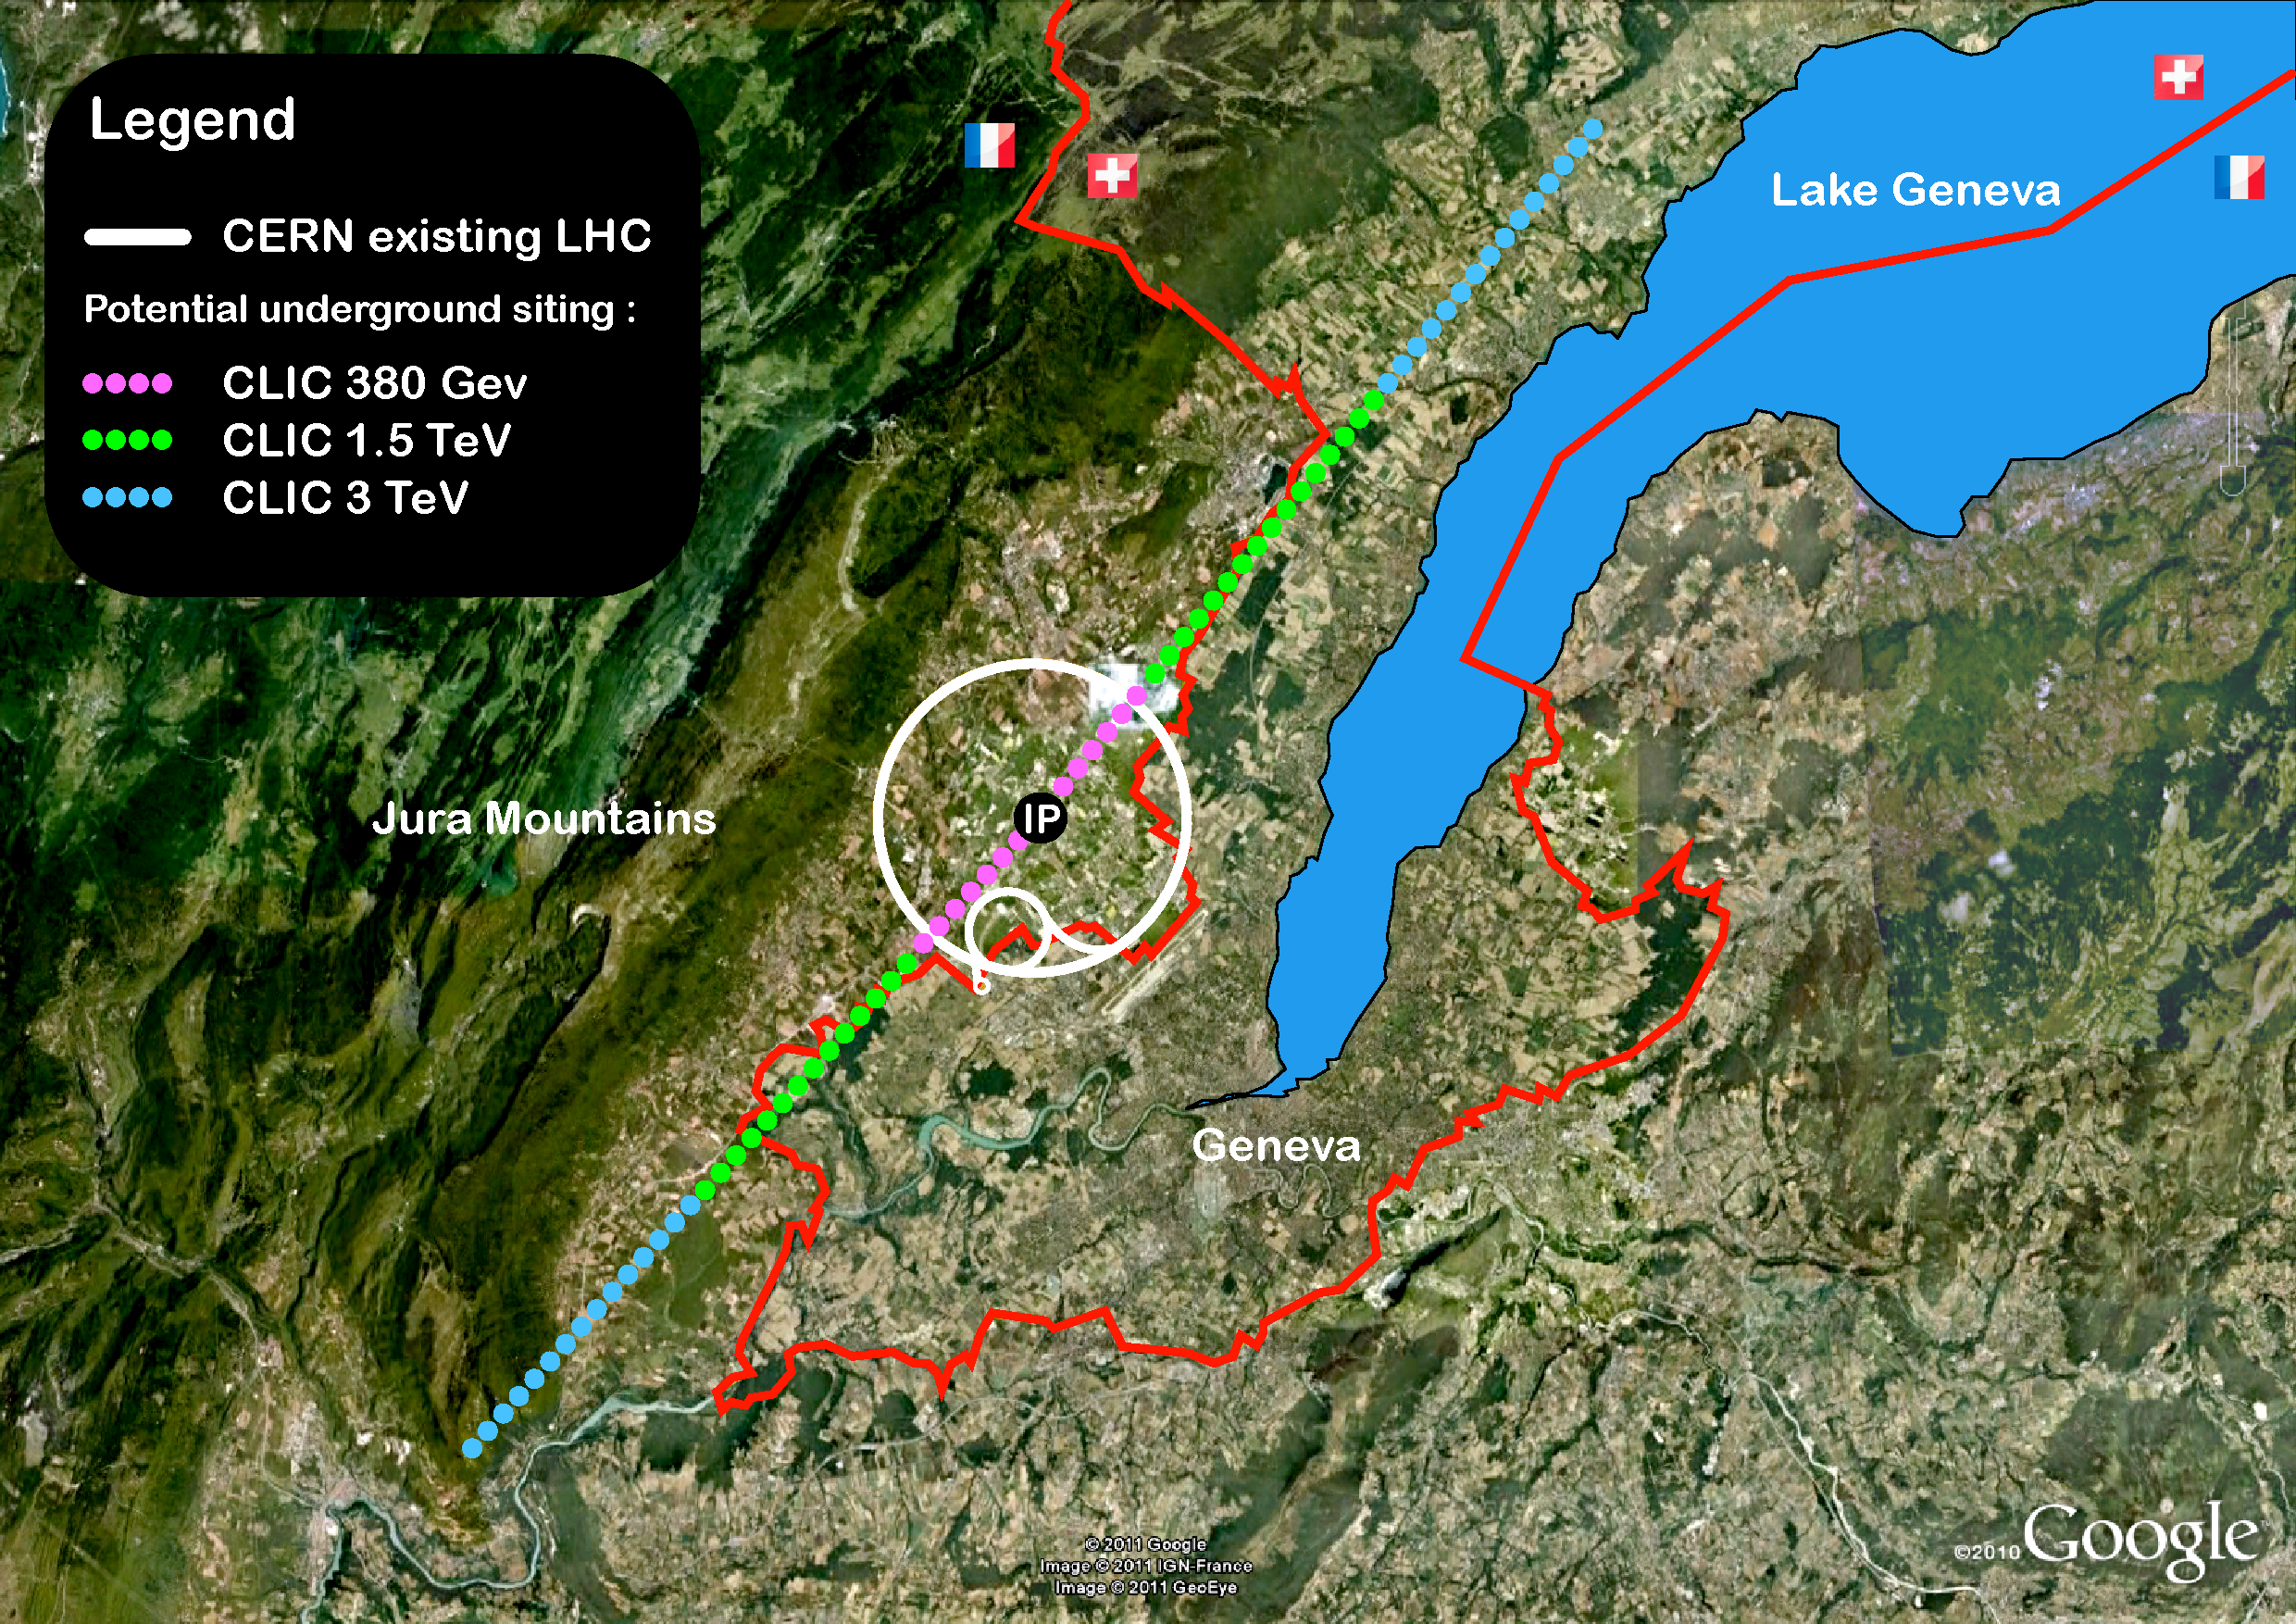
\includegraphics[width=0.7\textwidth]{figures/CLIC/staging.pdf}
  \caption{The three implementation stages of CLIC near CERN with
    center-of-mass energies of $380\,\gev$, $1.5\,\tev$ and
    $3\,\tev$~\cite{Felzmann:2157041}.}
  \label{fig:CLICstaging}
\end{figure}

The schematic layout of the CLIC accelerator complex at $3\,\tev$ is
shown in \cref{fig:CLIC_accelerator}. The electron and positron beams
are accelerated on a linear trajectory and collide in the central
region of the machine (in the interaction point), where the CLIC
detector is placed. At this stage, each linac is fed by a drive-beam
generation complex.

\begin{figure}[htbp]
  \centering
  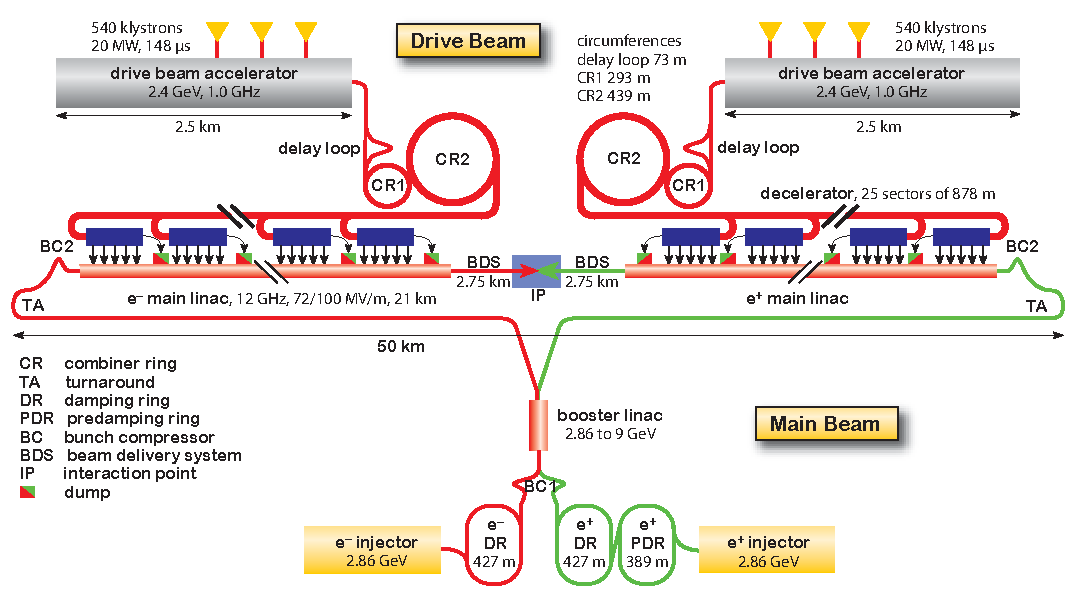
\includegraphics[width=\textwidth]{figures/CLIC/CLIC-layout2015pub.pdf}
  \caption{Schematic layout of the CLIC accelerator complex at
    $3\,\tev$~\cite{Felzmann:2157041}.}
  \label{fig:CLIC_accelerator}
\end{figure}


\section{The CLIC vertex-detector requirements}
\label{sec:VXD_requirements}

CLIC with its center-of-mass energies and instantaneous luminosity up
to $6\times10^{34}\,\inversecmsquaredsec$, allows for high precision
measurements of Standard Model physics (e.g. Higgs, top) as well as
new physics potentially discovered at the $13\,\tev$ LHC. One detector
concept covering the CLIC physics potential is under development in
simulations as shown in \cref{fig:CLIC_detector_concept}.

\begin{figure}[htbp]
  \centering
  \begin{tikzpicture}
    \node[anchor=south west,inner sep=0] (image) at
    (0,0){\includegraphics[width=0.62\textwidth]{figures/CLIC/CLICdp_Top_view_HD_temp.pdf}};
    \begin{scope}[x={(image.south east)},y={(image.north west)}]
      %% \draw[help lines,xstep=.1,ystep=.1] (0, 0) grid (1,1);
      %% \foreach \x in {0,1,...,9} { \node [anchor=north] at (\x/10,0) {0.\x}; }
      %% \foreach \y in {0,1,...,9} { \node [anchor=east] at (0,\y/10)
      %% {0.\y}; }
      \node[draw, text width=2cm] at (-0.2, 0.9) {Ultra low-mass vertex detector};
      \draw[->,line width=1pt, color=black](-0.02, 0.9) -- (0.5, 0.5);

      \node[draw, text width=2cm] at (-0.2, 0.7) {Main tracker, silicon based};
      \draw[->,line width=1pt, color=black](-0.02, 0.7) -- (0.35, 0.55);

      \node[draw, text width=2cm] at (-0.2, 0.5) {Forward region with LumiCal \& BeamCal};
      \draw[->,line width=1pt, color=black](-0.02, 0.45) -- (0.25, 0.49);

      \node[draw, text width=2cm] at (-0.2, 0.2) {Fine grained calorimetry used in Particle Flow (PFA)};
      \draw[->,line width=1pt, color=black](-0.02, 0.2) -- (0.3, 0.3);

      \node[draw, text width=2cm] at (1.15, 0.15) {Return yoke (Fe) with detectors for muon ID};
      \draw[->,line width=1pt, color=black](1, 0.1) -- (0.8, 0.1);

      \node[draw, text width=2cm] at (1.15, 0.5) {Solenoid magnet: B=4~T};
      \draw[->,line width=1pt, color=black](1, 0.45) -- (0.7, 0.21);
      

      \node[color=black] at (0.5, 0.05) {11.4~m};
      \draw[<->,line width=1pt, color=black](0.03, 0.02) -- (0.97, 0.02);
      
    \end{scope}
  \end{tikzpicture} 
  \caption{Schematic layout of the CLIC detector concept.}
  \label{fig:CLIC_detector_concept}
\end{figure}

A broad detector R\&D program at CLIC is addressing the challenging
experimental conditions and the demands for precision physics. This
thesis focuses on the vertex-detector R\&D.

The main goal of the CLIC vertex detector is the efficient tagging of
heavy quarks through the precise measurement of the displaced
vertices. To achieve this goal, Monte Carlo simulations have shown
that a high-momentum term in the transverse impact-parameter
resolution of $a\approx5\,\micron$ and a multiple-scattering term of
$b\approx15\,\micron$ are needed using the canonical parametrisation

\begin{equation}
 \sigma(d_0)=\sqrt{a^2+b^2 \cdot\gev^2/(p^2 \text{sin}^3\theta)} \; ,
  \label{eq:canonicalParam}
\end{equation}

where $p$ is the momentum of the particle and $\theta$ is the polar
angle with respect to the beam axis.

To meet these requirements, a multi-layer barrel and endcap pixel
detectors with an inner radius of $\approx$30~mm is needed. For the
beam-pipe and for each of the detection layers a material budget of
$\approx0.2\%$ of a radiation length (X\textsubscript{0}) is
considered. Sensors with a single-point resolution of
$\approx3\,\micron$ operating in a magnetic field of 4~T are required.

In the innermost layers, an occupancy of $\approx3\%$ due to the
beam-induced backgrounds are expected~\cite{Dannheim:1443516}. To
separate these backgrounds from physics events, a time slicing of the
hits with an accuracy of $\approx10$~ns is required.

In comparison to the current pixel detectors in the LHC experiments,
the exposure to radiation of the CLIC vertex detector is moderate. For
the inner-detector layers a total $1\,\mev$ neutron-equivalent fluence
of less than $10^{11}$~neq/cm\textsuperscript{2}/year and a total
ionising dose of less than 1~kGy are expected~\cite{Dannheim:1443516}.

The aim of the R\&D is to achieve the required single-point resolution
with pixels of size $\approx25\,\micron\times25\,\micron$ with
$50\,\micron$ thick sensors coupled to $50\,\micron$ thick analogue
readout ASICs. The constraint on the material budge implies no active
cooling elements can be placed inside the vertex detector. To limit
the maximum power dissipation of the readout electronics to
$\approx50~\text{mW/cm}^2$ forced air-flow cooling and power pulsing
(i.e. turning off most components on the readout chips during the
20~ms gaps between bunch trains) are foreseen.

\section{Flavour tagging performance at CLIC}
\label{sec:flavourTagging}

The precision physics measurements require excellent flavour-tagging
performance of the CLIC vertex detector. The flavour-tagging
performance is being investigated in simulations. The multi-variate
LCFIPlus flavour-tagging package~\cite{website:LCFIPlus} is used to
assign each jet category with a b- and c-probability.

The detector models in simulations considers the single-point
resolution of the sensors ($~3\,\micron$), constraints from the
mechanical support and the cooling
system~\cite{AlipourTehrani:1742993}.

As illustrated in Figure~\ref{fig:cooling}, a spiral arrangement for
the modules in the endcap regions can be used instead of disks,
allowing the air to flow through the vertex detector. The physics
performance of the geometries described in Table~\ref{tab:geometries}
and illustrated in Figure~\ref{fig:geometries} have been studied in
simulations.

\begin{table}[htbp]
  \caption{Geometries implemented in simulations.}
  \begin{center}
    \begin{tabular}{ l c c c }
      \hline
      Geometry & Barrel layers & Endcap layers & Material budget \\ \hline \hline
      \emph{spirals} (Figure~\ref{fig:SpiralsGeometry}) & 5 single-sided & 4 single-sided & $0.1\%X_{0}$ per single-sided layer  \\ %\hline 
      \emph{double\_spirals} (Figure~\ref{fig:doubleLayer}) & 3 double-sided & 3 double-sided & $0.2\%X_{0}$ per double-sided layer  \\ %\hline
      \emph{double\_spirals\_v2} & 3 double-sided & 3 double-sided & $0.4\%X_{0}$ per double-sided layer  \\ \hline  
    \end{tabular}
  \end{center}
  \label{tab:geometries}
\end{table}


\begin{figure}[htbp]
  \begin{subfigure}[b]{0.33\textwidth}
    \centering
    \includegraphics[width=\textwidth]{figures/CLIC/Cooling.png}  
    \caption{}
    \label{fig:cooling}
  \end{subfigure}~
  \begin{subfigure}[b]{0.33\textwidth}
    \centering
    \includegraphics[width=0.65\textwidth]{figures/CLIC/single_spiral.jpg}
    \caption{}
    \label{fig:SpiralsGeometry}
  \end{subfigure}~
  \begin{subfigure}[b]{0.25\textwidth}
    \centering
    \includegraphics[trim = 32mm 98mm 85mm 106mm, clip, width=0.65\textwidth]{figures/CLIC/double_spiral.pdf} \\
    \includegraphics[width=1.5\textwidth]{figures/CLIC/double_layer_module.png} 
    \caption{}
    \label{fig:doubleLayer}
  \end{subfigure}
  \caption{(a)~Sketch showing the airflow cooling strategy within the
    vertex detector~\cite{DuarteRamos:1572989}. (b)~Schematic view of
    the vertex detector for the \emph{spirals} geometry. (c)~Schematic
    view of the vertex detector for the
    \emph{double\_spirals(\_v2)}. In the \textsc{GEANT4} simulations,
    a double-sided layer is implemented as two silicon sensors on top
    of each other with an overall thickness of \SI{2}{\milli\meter}.}
  \label{fig:geometries}
\end{figure}

The performance of the flavour tagging depends on the jet energy and
polar angle: dijet events with different center-of-mass energies,
$\sqrt{s}$, having polar angles of $10^{\circ} \leq \theta \leq
90^{\circ}$ with a uniform distribution in $\phi$ angles are
considered. Initial state radiation (ISR) and beamstrahlung (BS) were
switched off during the event generation and hence the final-state
quarks are in a back-to-back configuration. For each jet flavour,
energy and angle, 80000 events are used for the following processes:
e$^+$e$^-$ $\rightarrow$ b\={b}, c\={c}, u\={u}, d\={d}, s\={s}. The
boosted decision trees (BDTs) are trained using 50\% of the generated
events and the other 50\% are used for testing the performance of the
flavour tagging.

The \emph{spirals} and \emph{disks} have a similar flavour-tagging
performance except for jets at $\theta=40^{\circ}$ (see
Figure~\ref{fig:spiral_disks}), which corresponds to the transition
between the vertex endcaps and the barrel region, where the
beauty-tagging performance is up to $20\%$ worse using the
\emph{spirals} geometry (compared to disks). With the spiral
configuration, the number of sensitive layers becomes dependent on the
azimuthal angle $\phi$ and less layers can be hit in certain ranges of
$\phi$. The performance of the \emph{spirals} and the
\emph{double\_spirals} is very similar as shown in
Figure~\ref{fig:spiral_doubleSpirals}.  The \emph{double\_spirals\_v2}
geometry is a more realistic version of the \emph{double\_spirals}
geometry, taking into account the material used for the mechanical
support of the sensors and also for the cables. As shown in
Figure~\ref{fig:doubleSpirals_doubleSpirals}, the misidentification
probability increases by $\sim$35\% due to the increased material.


\begin{figure}[htbp]
  \begin{subfigure}[b]{0.33\textwidth}
    \centering
    \begin{tikzpicture}
      \node[anchor=south west, inner sep=0] (image) at (0,0){\includegraphics[trim = 5mm 50mm 20mm 20mm, clip, width=\textwidth]{figures/CLIC/200GeV_Ratio_allAngles_spirals_CDR_B_C.pdf}};
      \draw  (1.8, 1.5) node {\textbf{CLICdp}};
    \end{tikzpicture}
    \caption{}
    \label{fig:spiral_disks}
  \end{subfigure}~
  \begin{subfigure}[b]{0.33\textwidth}
    \centering
    \begin{tikzpicture}
      \node[anchor=south west, inner sep=0] (image) at (0,0){\includegraphics[width=\textwidth]{figures/CLIC/general_200_Beauty.pdf}};
      \draw (1.8, 2.8) node {\textbf{CLICdp}};
    \end{tikzpicture}
    \caption{}
    \label{fig:spiral_doubleSpirals}
  \end{subfigure}~
  \begin{subfigure}[b]{0.33\textwidth}
    \centering
    \begin{tikzpicture}
      \node[anchor=south west, inner sep=0] (image) at (0,0){\includegraphics[width=\textwidth]{figures/CLIC/heavy_general_200_Beauty.pdf}};
      \draw (1.8, 2.8) node {\textbf{CLICdp}};
    \end{tikzpicture}
    \caption{}
    \label{fig:doubleSpirals_doubleSpirals}
  \end{subfigure}
  \caption{Beauty-tagging performance for dijet events at
    \SI{200}{\giga\electronvolt}. (a)~Comparison between \emph{disks}
    and \emph{spirals} in terms of the ratio of the misidentification
    probabilities for charm background. (b)~Comparison of the
    beauty-tagging performance between the \emph{spirals} and
    \emph{double\_spirals} geometries. (c)~Comparison of the
    beauty-tagging performance between the \emph{double\_spirals} and
    \emph{double\_spirals\_v2} geometries. For (b) and (c), dijet
    events with a mixture of polar angles between \SI{10}{\degree} and
    \SI{90}{\degree} are considered.}
  \label{fig:performance}
\end{figure}

% In the following Section, we describe different components of the CLIC detector.
% %%%%%%%%%%%%%%%%%%%%%%%%%%%%%%%%%%%
% %             Section             %
% %%%%%%%%%%%%%%%%%%%%%%%%%%%%%%%%%%%
% \section{The CLIC\_SiD Detector Concept} \label{sec:DetectorDesign}

% Figure \ref{fig:CLIC3tev} shows the layout of the CLIC accelerator for a center-of-mass energy of 3~TeV. The electron and positron beams are accelerated on a linear trajectory and collide in the central region of the machine (in the interaction point), where the CLIC detector is placed.
% % \begin{figure}[H]
% %   \centering
% %   \includegraphics[page=2, trim=20mm 35mm 0mm 180mm, clip, width=0.85\textheight]{Chapters/Figures/CLIC/clicLinearColliderStudies}
% %   \caption{The schematic view of the CLIC layout for a center-of-mass energy of 3~TeV. From~\cite{CLICLinssen2012}.}
% %   \label{fig:CLIC3tev}
% % \end{figure}
% The site studies have shown that CLIC could be placed near CERN underground as shown in Figure \ref{fig:CLICfootprint}. It shows how CLIC could be built in stages. For each energy increase more accelerating modules will be needed, making the accelerator longer. The site length for 3~TeV will be 48~km. 
% % \begin{figure}[H]
% %   \centering
% %   %\hspace{-0.3cm}
% %   \includegraphics[page=3, trim=40mm 180mm 40mm 10mm, clip, width=0.7\textwidth]{Chapters/Figures/CLIC/clicLinearColliderStudies}
% %   \caption{CLIC footprint near CERN, for different implementation stages. From~\cite{CLICLinssen2012}.}
% %   \label{fig:CLICfootprint}
% % \end{figure}
% The CLIC detector model studied in this thesis is called  CLIC\_SiD which is based on the SiD detector concept \cite{SiDAihara:2009ad} developed for the International Linear Collider (ILC) \cite{Brau:2007zza}. ILC is another linear e$^+$e$^-$ collider under development. It is based on a different acceleration technique. ILC can reach 500~GeV center-of-mass energy for a site length of 32~km, while CLIC can reach 3~TeV for a site length of 48~km. The ILC may be implemented in Japan. \\
% The SiD detector is considered as a compact detector with an overall length of 12.39~m and a total height of 12.50~m. It is composed of several sub detectors. Its main components are shown in Figures \ref{fig:CLIC_SiD_model} and \ref{fig:CLICcomponents} and briefly described in the following sections.


% % \begin{figure}[H]
% %   \centering
% %   %\hspace{-3cm}
% %   %\includegraphics[page=32, trim=30mm 180mm 10mm 20mm, clip, width=0.75\textheight]{Chapters/Figures/CLIC/clicCDR_vol3.pdf}
% %   \includegraphics[angle=-90,width=0.8\textwidth]{Chapters/Figures/CLIC/3D.pdf}
% %   \caption{The CLIC detector model. The beams come from the two sides of the detector and collide at its center in the Interaction Point (IP). From \cite{CLICCDRvol3}.}
% %   \label{fig:CLIC_SiD_model}
% % \end{figure}

% % \begin{figure}[H]
% %   \centering
% %   %\hspace{-3cm}
% %   \includegraphics[page=3, trim=30mm 165mm 0mm 50mm, clip, width=0.75\textwidth]{Chapters/Figures/CLIC/LCD-2011-009.pdf}
% %   \caption{One quadrant of the CLIC\_SiD detector model in the xy-plane (left) and in the zx-plane (right). Distances are given in millimeters. From \cite{Grefe2011}.}
% %   \label{fig:CLICcomponents}
% % \end{figure}


% %%%%%%%%%%%%%%%%%%%%%%%%%%%%%%%%%%%
% %           subection             %
% %%%%%%%%%%%%%%%%%%%%%%%%%%%%%%%%%%%


% %-------------------------------------

% \subsection{Tracking Detectors} \label{sec:VertexDetectorBarrel}

% The tracking system consists of silicon detectors with excellent point resolution and low material budget placed in the innermost part of the detector and very close to the interaction point. It covers a wide range of polar angles and the lowest angle measured is for $\theta = 8^\circ$. The tracking system is made of two main components: the vertex detector  and the main tracking system which are detailed in the sections below.\\
% The tracker measures the position of the charged particles in several layers and allows for the precise measurement of particle trajectories. The measurement of the curvature of the track yields very precise information on the particle's momentum (cf. Equation \ref{eq:curvatureRadius}). \\
% The vertex detector uses silicon pixel detectors while the main tracking system uses silicon microstrip detectors. In the region close to the interaction point, the density of the particles is very high. To measure the position of the charged particles with a high precision, the pixels provide a high spatial resolution. But they need a complex readout system and they are very expensive. For these reasons, they are used only at the inner part of the detector. \\
% The main tracking system consists of silicon microstrip detectors. The strips are placed along a specific direction. In order to have the coordinates of a particle hit, two strips with two different directions are used. The overlap between the strips provides the position of the hit in the detector. But the strips can not provide precise measurements when the density of the particles is high because many strips can be activated which corresponds to many overlaps between the strips. For this reason, they are placed in the regions further away from the interaction point. They need a simpler readout system compared to the pixel detectors and they are more cost-effective. \\
% Also particles with higher momentum reach the region covered by the tracking system and their radius of curvature is lower in the magnetic field and they have a more linear trajectory. Silicon strips give enough precision on their track reconstruction. The pixel detectors improve the precision of the track reconstruction for low-momentum particles as they bend more in the magnetic field.\\
% \subsubsection{Vertex Barrel and Endcap} \label{sec:vertexDet}
% The vertex barrel is composed of five concentric layers each made of several modules. The vertex endcaps cover the forward region close to the interaction point of the detector and is composed of four disks each made of several trapezoidal modules. The vertex barrel and endcaps are described in detail in Section \ref{sec:defaultGeom}. 
% Each module contains a silicon sensor with a thickness of \(50\ \mu \)m and with a pixel size of \SI{25}{\micro\metre}$\times$\SI{25}{\micro\metre}. The single-point accuracy obtained is \SI{3}{\micro\metre}. The silicon sensor is the sensitive part of each module. In Section \ref{sec:radiationDetection}, an introduction on silicon sensors is given. Figure \ref{fig:vertex3D} illustrates the vertex barrel and endcaps for the CLIC\_SiD as defined in \cite{CLICCDR2012}.

% % \begin{figure}[H]
% %   \centering
% %   \begin{tikzpicture}
% %     \node[anchor=south west,inner sep=0] (image) at (0,0){\includegraphics[width=0.6\textwidth]{Chapters/Figures/Geometries/views/VXD_Barrel_and_Disks.png}};
% %     \begin{scope}[x={(image.south east)},y={(image.north west)}]
% %       \draw[black, <->, thick] (0.37, 0.73) -- (0.56, 0.79);
% %       \node[above, text=black] at (0.47, 0.8){20~cm};

% %       \draw[black, ->, thick] (1., 0.25) -- (0.9, 0.45);
% %       \node[below, text=black] at (1.1, 0.23){Beam pipe};

% %       \draw[black, ->, thick] (0.85, 0.2) -- (0.75, 0.4);
% %       \node[below, text=black] at (0.85, 0.2){Vertex disks};

% %       \draw[black, ->, thick] (0.55, 0.2) -- (0.45, 0.4);
% %       \node[below, text=black] at (0.55, 0.2){Vertex barrel};
% %     \end{scope}
% %   \end{tikzpicture}
% %   \caption{Schematic picture of the vertex barrel and endcaps. For CLIC\_SiD, the barrel contains five layers and the endcaps are made of four disks of silicon pixel detectors.}
% %   \label{fig:vertex3D}
% % \end{figure}


% \subsubsection{Tracker Barrel and Tracker Endcap} \label{sec:VertexTracker}

% The tracker barrel surrounds the vertex detector. It contains five layers of silicon microstrip detectors. The tracker endcap covers the forward region with four concentric disks (after the vertex endcaps) as shown in Figure \ref{fig:tracking}. \\
% The silicon microstrip detectors have a typical strip length of \SI{10}{\centi\metre} and a strip pitch of \SI{50}{\micro\metre}. The typical measurement accuracy for single hits is approximately \SI{7}{\micro\metre} in the bending plane.

% % \begin{figure}[H]
% %   \hspace{-3cm}
% %   \includegraphics[page=7, trim=0mm 163mm 10mm 50mm, clip, width=0.8\textheight]{Chapters/Figures/CLIC/LCD-2011-009.pdf}
% %   \caption{The layout of the tracking system in the xy-plane (a) and in the zx-plane (b). The tracker modules are shown in yellow and the support structures in brown. All distances are given in millimeters. From \cite{Grefe2011}.}
% %   \label{fig:tracking}
% % \end{figure}

% \subsection{Calorimeters}
% Calorimeters are placed after the tracking systems. Two types of them are used: the silicon-tungsten electromagnetic calorimeter (ECAL) and the hadronic calorimeter (HCAL). The calorimeters are used to measure the energy of the particles. The ECAL is designed to measure the energy of particles interacting via the electromagnetic interactions and the HCAL is aimed at measuring particles interacting via the strong nuclear force. 


% \subsection{Superconducting Coil}
% The superconducting coil provides a solenoidal magnetic field of 5~T. It is placed outside of the calorimeters. The magnetic field deflects the trajectory of charged particles. Tracking detectors use the radius of curvature to measure the momenta of charged particles (cf. Section \ref{sec:resolution_spiralEndcaps}).


% \subsection{Iron Yoke}
% The iron yoke surrounds the whole detector. It forms an integral part of the magnet system and contains detection layers to identify the muons. 



% %%%%%%%%%%%%%%%%%%%%%%%%%%%%%%%%%%%
% %             Section             %
% %%%%%%%%%%%%%%%%%%%%%%%%%%%%%%%%%%%

% \section{Introduction to Silicon Detectors for the Tracking System} \label{sec:radiationDetection}

% The tracking detectors are made of silicon detectors. A silicon atom has four electrons in the valence band. In the fundamental state of a semi-conductor, the conduction band is empty and behaves like an insulator. When the energy of the electrons raises by thermal excitation or energy absorption, they can jump from the valence band to the conduction band. The \begin{it}band gap\end{it} between the valence and the conduction band is 3.62~eV (at 300~K) \cite{knoll2000radiation}. When an electron moves from the valence to the conduction band, it leaves behind a hole representing a positive charge. This hole can be filled by an electron from a neighboring atom. The electric conduction is then generated by the electron-hole displacement. \\
% By introducing impurities, like doping the silicon with atoms having five valence electrons, an n-type silicon is obtained. Indeed, the fifth electron from the impurity can jump easily in the conduction band. A p-type silicon is obtained by doping with silicon atoms having three valence electrons.
% By creating a junction between a p-type and an n-type silicon, the electrons from the n-type silicon move to the p-type side and holes move in the opposite direction. This charge movement continues until a balance is created and no charge moves. A \begin{it}depletion\end{it} zone is created which stops the conduction between the two areas. By applying a voltage between the two sides of the junction where the n side is negative compared to the p side, the junction conducts the current. 
% The depletion zone can be increased by applying a positive voltage to the n side compared to the p side. This configuration is shown in Figure \ref{fig:SiliconDetector}.\\ 
% Indeed, in such a system, when a high-energy charged particle goes through the depletion zone, it produces electron-hole pairs by losing its energy. The Bethe-Bloch equation \cite{Balbuena:1511878} gives the rate of ionizing loss of a charged particle in matter. For high-energy particles (at energies above several hundred MeV) having velocities approaching the speed of light, the energy loss approaches a constant minimum value. \begin{it}Minimum ionizing particles\end{it} (MIP) refers to relativistic particles with high velocities and they have the same energy loss behavior in matter. But for a non relativistic charged particles ($v \ll c$), the energy loss varies inversely with particle energy as they spend greater time in matter. \\
% In the existing tracking systems, silicon sensors with a thickness of \SI{300}{\micro\meter} are used which provide around 20000 electron-hole pairs. CLIC requires very low material in the tracking system. Based on the studies done in \cite{CLICCDR2012}, the silicon sensor has to have a thickness of \SI{100}{\micro\meter} which provides around 7000 electron-hole pairs. In this case, the readout system has to be very precise with a high noise rejection.\\
% As a voltage is applied to the both sided of the p-n junction, the created charge moves out of the depleted zone and a detectable electrical current is generated. Then the generated current is measured using readout pads. In the vertex barrel and endcaps areas close to the beam pipe, small pixels are used as readout pads. For a depleted detector, the speed of charge collection is a few~ns which allows the use of a high rate readout system. \\


% ============================================================================== 
% planning for the chapter
% ============================================================================== 
% Accelerator (two-beam acceleration), CLIC detector concept, picture of
% the full detector (3 pages)

% \section{Requirements for the CLIC vertex detector}
% motivation for pixel detectors in high-energy physics (flavour-tagging
% plots), requirements, design, technical challenges
% (cooling/mechanics), Beam induced backgrounds, Radiation damage in the
% vertex detector (3 pages).


% \section{Flavour tagging at CLIC}
% say motivation of this thesis $\Rightarrow$ provide input for the
% digitiser (1 page) and the detector simulation software.
